\documentclass{article}
\usepackage{float}
\usepackage{lipsum}
\usepackage[utf8]{inputenc}
\usepackage[smartEllipses]{markdown}
\usepackage[newfloat]{minted}
\usepackage{caption}
\usepackage[parfill]{parskip}
\usepackage{hyperref}
%\usepackage[obeyspaces]{url}
\newenvironment{code}{\captionsetup{type=listing}}{}
\SetupFloatingEnvironment{listing}{name=Code}

\title{The installation, configuration and use of QFieldCloud}
\author{Pettersson, E. Jussila, A. Chau, N}
\date{29.11.2021}

\begin{document}

\maketitle

\tableofcontents

\pagebreak
\section{Introduction}
The aim of the project was to investigate the state of QFieldCloud by conducting Proof-of-Concept testing. The project was commissioned by the National Land Survey as a study project in Aalto University. With the project, we gain more understanding of the possibilities that self-hosted QFieldCloud could provide together with other applications, such as QGIS software and QField mobile GIS app. The motivation of this project comes from the development of the National Land Survey's maintenance system for Topographic Database.

QFieldCloud is an open-source software by OPENGIS.ch. Therefore, it is freely available for everyone to use and modify. The software is a Django-based service to synchronize projects and data between QGIS with QFieldSync-plugin and QField. 

The mentioned technologies can be used for example by the field surveyors to update data with mobile devices to QFieldCloud. After that the new data can be exported from QFieldCloud to Topographic Database (PostGIS) or QGIS for managing the data. In short, QFieldCloud aims to provide seamless synchronization to make workflow better in maintenance of spatial infrastructure with version control, team management and online--offline work options in QField. 

\begin{markdown}
This project report, example project and the NLS data used in the project can be found from our [Github repository](https://github.com/gis-e6010-qfieldcloud/qfieldcloud-aalto-demo) along with the PostgreSQL dumps that can be used to generate NLS geodata from the Helsinki region. The repository also contains a fork of the QFieldCloud which does not contain any changes by us, but is effectively a frozen-in-time version of the QFieldCloud as we used to use it.  
\end{markdown}

% Ngoc
\section{Installation of QFieldCloud}\label{sec:install}
\begin{markdown}
___Disclaimer: The report is written based on a version of QFieldCloud which most closely corresponds to tag v0.12.0 in the official QFieldCloud Github-repository. For example, the most up-to-date version at the time of writing this manual (Dec 12th, 2021) has completely removed the Caddy server and uses NGinx server instead. As the project is moving so fast, it might be hard to keep up with the changes and therefore the documentation on the official repository is also sometimes lagging behind. The client software might also be suspected to changes.___

Before installing the QFieldCloud, make sure that you have [Git](https://git-scm.com/) on your server. You can create a new folder to a directory where you want to download the data to. The repository of QFieldCloud can be found here:
\end{markdown} 
\url{https://github.com/opengisch/qfieldcloud}. 
\begin{markdown}
Use git clone command to copy the files from the remote repository to your current directory. Configure your environment by setting the environment variables in the ```.env.example``` file as you wish before building your QFieldCloud instance. 

The ```.env.example``` file consist of different environment variables that can be changed according to your own setup. For example, you can change the variable ```QFIELDCLOUD_HOST``` to the public IP address of the server if you want the service to be found on the public network. You can also configure the S3 object storage either to be an internal ([MiniO](https://min.io/)) or external storage ([AWS S3](https://aws.amazon.com/s3/)) from the mentioned file.
\end{markdown}
See more information in the section \ref{sec:Components}.

When the environment configuration is done, you can build your instance by docker-compose which is a tool for running multi-container Docker applications. Keep in mind that the QFieldCloud is using the port 8000, and make sure that the port is not used by anything else. This also goes for other ports used by different components. Type the following commands into the terminal to build the local instance on your server:

\begin{minted}[breaklines]{sh}
# Git clone QFieldCloud repository to current folder
git clone https://github.com/opengisch/qfieldcloud.git --recursive

# Copy the `.env.example` into `.env` file and configure it 
# with an editor that you are comfortable with:
cp .env.example .env

# Run and build the docker containers
# It will start the Django built-in server 
# at http://localhost:8000 (if QFIELDCLOUD_HOST is not changed) 
docker-compose -f docker-compose.yml -f docker-compose.override.local.yml up -d --build

# Collect the static files (CSS, JS, etc.)
docker-compose run app python manage.py collectstatic --noinput

# Run the Django database migrations
docker-compose -f docker-compose.yml exec app python manage.py migrate

# Check the status via manage.py script. 
# If everything has been done properly, 
# redis, geodb and storage should checked as 'ok'.
docker-compose run app python manage.py status
\end{minted}

\begin{markdown}
Now you should have the QFieldCloud local instance running and you can access the admin page at http://yourIPaddress:8000/admin/login. In order to login the admin page, you need to create a ```superuser``` by the following command:
\end{markdown}
\begin{minted}{sh}
# Replace the username and email as you want
# After entering the command it will ask you to create a password
docker-compose run app python manage.py createsuperuser
--username super_user --email super@user.com
\end{minted}

\subsection{Docker and docker-compose}
\begin{markdown}
In the installation of QFieldCloud, we are using Docker since the software has been containerized by the mentioned technology. Docker helps in packaging applications and its dependencies in containers. This makes it easy to deploy applications in different computing environments. Containers isolate the software from its environment and make sure that the software works as the same despite any possible differences. In addition to Docker, we need [Docker-compose tool](https://docs.docker.com/compose/) since we are dealing with multi-container Docker application.

### Install Docker
Docker can be installed using Ubuntu’s default repository or Docker’s official repository. Installing from default repository is the easiest way to install docker. This method consists of single line, which is *sudo apt-get install docker*. Though this method does not provide the latest version of Docker. Latest version can be installed via the official repository. In this method some preliminary settings have to be done before installation. 

To set up the repository the apt package index should be updated and packages that allow apt to use repositories over HTTPS should be installed. After this Docker’s official GPG key is added. The last step is to set up the official repository. Then, the only thing remaining is the installation of Docker and Docker-compose.
\end{markdown}

\begin{minted}[breaklines]{sh}
# Update apt package index 
#and allow apt use repositories over HTTPS:
sudo apt-get install apt-transport-https ca-certificates curl gnupg lsb-release

# Add Docker’s official GPG key 
#(Ubuntu needs to have curl installed)
curl -fsSL https://download.docker.com/linux/ubuntu/gpg | sudo gpg --dearmor -o /usr/share/keyrings/docker-archive-keyring.gpg
\end{minted}

\begin{minted}[breaklines]{sh}
# Set up the repository
echo "deb [arch=$(dpkg --print-architecture) signed-by=/usr/share/keyrings/docker-archive-keyring.gpg] https://download.docker.com/linux/ubuntu $(lsb_release -cs) stable" | sudo tee /etc/apt/sources.list.d/docker.list > /dev/null

# Update the apt package index
sudo apt-get update

# Installation of docker components
sudo apt-get install docker-ce docker-ce-cli containerd.io
\end{minted}

\begin{markdown}
### Install Docker-compose
Docker-compose can be installed through default repository or manually. The simplest way is to use default repository and install via command *sudo apt-get install docker-compose*. The files can also be downloaded manually using curl. The permission has to be added so that the program is able to work properly. Optionally one can also add a symbolic link to the docker compose installation directory.
\end{markdown}

\begin{minted}[breaklines]{sh}
# Download current stable release of Docker Compose:
sudo curl -L "https://github.com/docker/compose/releases/download/1.29.2/docker-compose-$(uname -s)-$(uname -m)" -o /usr/local/bin/docker-compose

# Apply executable permissions to the binary
sudo chmod +x /usr/local/bin/docker-compose

# Create a symbiotic link to /usr/bin
sudo ln -s /usr/local/bin/docker-compose /usr/bin/docker-compose

\end{minted}


\subsection{Installation of VirtualBox with Ubuntu}
\begin{markdown}
If you would like to install QFieldCloud on your computer, it is preferable to have Ubuntu operating system. QFieldCloud is designed to work in Linux distribution. You can install it easily with VirtualBox. VirtualBox is open-source software used for virtualization. It allows to run multiple operating systems inside a host computer. VirtualBox can be downloaded from the developers website (www.virtualbox.org). The version used in this project is 6.1.26 package for Windows 10. The location of the software should be chosen so that there is enough disk to save the running operating systems.

To create a virtual machine one needs an operating system file which is the Ubuntu Linux distribution. Ubuntu can be downloaded from this [link](https://ubuntu.com/download/desktop). The most stable and current release is 20.04 LTS, which is chosen for this project. After downloading one should have a Ubuntu file that ends in .iso.

Next, the new Virtual Machine should be created in Virtual Box. Give the virtual machine a name and choose the location of the installation. Linux is set as type and Ubuntu (64-bit) as version. Now comes for the allocation of memory. It is generally recommended to not allocate over 50 % of your host machines resources (e.g. maximum ram 16 GB, allocated ram 8 GB). In Hard disk settings select 'Create a virtual hard disk now'. In hard disk file type VDI should be selected. At 'Storage on physical hard disk' one can choose dynamic or fixed size. Either one works. Then file location directory and hard disk size is set. In this case 50 GB should be enough.

Now there should be a new instance on the left panel of VirtualBox. The name of the is the name of the virtual machine that was given before. Next, Linux Ubuntu will be installed using the ISO file that was downloaded earlier. Select instance’s settings and go to storage, where the ISO file is added to Controller: IDE. Next, start the virtual machine. In the select start-up disk choose the Ubuntu 20.04 LTS ISO file and press start. After that follow the instructions and select your preferred language and keyboard layout.

### Updating Ubuntu
Ubuntu should always be updated and upgraded before installing new programs. There are a lot of tools that can be installed quite easy because of the Linux repository. It is recommended installing curl, zip, unzip. Ubuntu should also always be updated if repository is modified. Otherwise, the installation of programs via apt-get install will not work.
\end{markdown}

% Eemeli
\subsection{Installation on RedHat Enterprise Linux 8 Server}
\subsubsection{The prerequisites on the RedHat Enterprise Linux 8}\label{sec:serverEnv}
\begin{markdown}
Let us first introduce the server environment. The server we were offered by Aalto University was a x86-64 based virtual machine running RedHat Enterprise Linux 8 (later RHEL 8). We were allocated one core of a *Intel(R) Xeon(R) CPU E5-2680 v4* running at 2.40GHz and the machine had 2GB of RAM. The processing capacity was more than sufficient but it is essential to realize that the CPU was x86-64 based as beginning from RHEL 8, Docker (and RedHat) discontinued official support on x86-64-based CPUs. Therefore, the Docker cannot be downloaded from the official Docker repository and we had to use CentOS repository instead. There's an official version of Docker available for RHEL 7 and RHEL 8 for s390x (IBM Z) CPU architecture. Consider using either of those or move to Podman, which RedHat recommends, or Kubernetes, if you are using RHEL 8.

The lack of official support, on the other hand, makes our server solution little less robust than using the official Docker from the company repository but, on the other hand, makes the process of installing everything likely work on other distributions using RPM package management, such as CentOS, Fedora and Mandriva, though those weren't tested. It is still safest to state that the following instructions will only apply to RHEL 8 and Oracle Linux 8.   

The installation process on RedHat Enterprise Linux 8 differs somewhat from the process on Debian-based Linux distributions such as Ubuntu described in the last section. The process was first tested using Oracle Linux Server 8, which is essentially RedHat Enterprise Linux 8 with RedHat branding and exclusive parts removed and some added Oracle branding and tools.  

The Docker can be installed from CentOS repository by first adding the repository to the list of package repositories using *dnf configmanager*, then removing any conflicting packages using *dnf* and installing the *docker.ce* and other components from the newly added repository. Those commands can be found below:   
\end{markdown}
\begin{minted}{sh}
# We had to first install tools such as "zip" and "unzip" 
# and "git" as our server came with very limited set of
# tools installed by default.
sudo dnf install -y dnf-utils zip unzip
sudo yum install git
# Then add the repository
sudo dnf config-manager \
--add-repo=https://download.docker.com/linux/centos/docker-ce.repo
# Remove packages that might conflict with the Docker
sudo dnf remove -y runc
# Install Docker from the repository
sudo dnf install -y docker-ce --nobest
\end{minted}

\begin{markdown}
After the last set of commands you should have Docker installed on the machine. However, unlike on Debian-based distributions, the *docker.service* does not start by default and will have to be elevated as a service with Systemd. Before that, it's recommended to add your user to *docker* group. _In RHEL 8, this has to be run from root shell or equivalent (`sudo -i`), The `sudo` before the command does not work. You can do this in the following way:
\end{markdown}

\begin{minted}{sh}
# From ROOT shell (e.g. sudo -i)
# Add docker group
groupadd docker
# Add current user (with sudo rights) to the docker group
usermod -aG docker $USER
# Enable service (non-ROOT shell)
systemctl enable docker
# Start the service (non-ROOT shell)
systemctl start docker
\end{minted}

\textbf{Warning: Adding sudoer to docker group essentially grants \texttt{docker} superuser privileges. However, superuser privileges are needed to run \texttt{docker} and without them rights Docker can not restart your containers if they crash for some reason. We found this the hard way. There are also some Docker-related commands which work in root shell and after adding sudoer to docker group but not with plain \texttt{sudo} command. Having the need to give \texttt{docker} superuser privileges is one of the main arguments against using \texttt{docker} in security-oriented applications.}

\begin{markdown}
You should then check the status of the service and Docker using
\end{markdown}
\begin{minted}{sh}
systemctl status docker.service
\end{minted}

which should contain lines such as
\begin{minted}{sh}
Loaded: loaded (/usr/lib/systemd/system/docker.service; enabled; \ 
vendor pres>
Active: active (running) since Wed 2021-12-01 03:42:47 EET; 15h ago
\end{minted}

It's equally good idea to check the functioning of Docker using the good old \texttt{hello-world} with
\begin{minted}{sh}
sudo docker run hello-world
\end{minted}
which should download the respective image from Docker container image library \emph{Docker Hub}, build the container and run it. If you don't get any error messages, your Docker daemon is most likely running correctly. 

In addition to Docker, we also need \texttt{docker-compose} to build the \emph{QFieldCloud} application. On RHEL the \texttt{docker-compose} can be installed with
\begin{minted}{sh}
sudo curl -L \ 
"https://<github-url>/docker-compose-$(uname -s)-$(uname -m)" \ 
-o /usr/local/bin/docker-compose
\end{minted}
where
\begin{minted}{sh}
sudo curl -L \ 
github-url = 
github.com/docker/compose/releases/download/1.29.2
\end{minted}
\begin{markdown}
points to the release you wan't to use. The `$(uname -s)` command automatically points to your operating system kernel, in our case *Linux*, `$(uname -m)` to your CPU architecture (e.g. *x86_64*), The binary corresponding to the right kernel and architecture is copied to `/usr/local/bin/docker-compose` directory and given execution rights with

```sudo chmod +x /usr/local/bin/docker-compose
```
Then just create a symbolic link to `/usr/bin/docker-compose` with

```sudo ln -s /usr/local/bin/docker-compose /usr/bin/docker-compose
```
\end{markdown}

Now you should have both \textbf{docker} and \textbf{docker-compose} installed and ready to use. 

\subsubsection{Installing QfieldCloud development server}
The actual installation process of QFieldCloud on the server is very similar to the one described in Section \ref{sec:install} but instead of the local instance, a server development instance was built. Therefore, these instruction assume that you have the repository cloned and the software installed as described in the previous section. 

For the development server instance, we had to create an Amazon S3 bucket since the \texttt{.yml} file (\texttt{docker-compose.override.dev.yml}) for the development server instance doesn't contain build instructions for the local MiniO storage and assumes an external storage bucket be used instead. It would also be possible to use external MiniO or some other S3 protocol implementation, but we decided to use Amazon S3 as it was free of charge and we could get a working bucket in matter of few hours including all the research that went into making it work. 

In order to get a suitable bucket from Amazon AWS, you have to first create an S3 bucket \textbf{with versioning enabled} with AWS Console or AWS-CLI, then an IAM user with access key and secret key, which you should store somewhere safe and assign to \texttt{STORAGE\_ACCESS\_KEY\_ID} environmental variable. The secret key to that IAM should be assigned to the \texttt{STORAGE\_SECRET\_ACCESS\_KEY} To that user, you should attach the \texttt{AmazonS3FullAccess} policy, which allows full access to S3 buckets on that account with that specific IAM user. Then in the \texttt{.env} file specify

\begin{minted}[breaklines]{sh}
STORAGE_ACCESS_KEY_ID=<Key ID of IAM user with S3FullAccess policy>
STORAGE_SECRET_ACCESS_KEY=<Secret access key for IAM user>
STORAGE_BUCKET_NAME=<name for your AWS S3 bucket>
STORAGE_REGION_NAME=<AWS region where your bucket is hosted>
# Internal URL to the storage endpoint (from python code)
STORAGE_ENDPOINT_URL=<S3 storage access endpoint>
# Public URL to the storage endpoint (external storage should be equivalent to STORAGE_ENDPOINT_URL, local development only, no trailing slash)
STORAGE_ENDPOINT_URL_EXTERNAL=<S3 storage access endpoint>
\end{minted}

After setting up the \texttt{.env} file, you can start building the development server. Rename the \texttt{.env.example} to \texttt{.env} if you already haven't done that. 

\begin{minted}[breaklines]{sh}
# Create a directory for the server logs
mkdir /var/local/qfieldcloud
# Build the development server
docker-compose -f docker-compose.yml -f \ 
docker-compose.override.dev.yml up -d --build
\end{minted}

If the build completed succesfully and
\begin{minted}[breaklines]{sh}
docker-compose run app python manage.py status 
\end{minted}
outputs OK for every category, you should have a working development server.

\begin{markdown}
__Attention: In some cases, the script may return "storage: error" but the storage is still working. This may have something to do how the existence of the bucket is checked in the [status](https://github.com/opengisch/qfieldcloud/blob/master/docker-app/qfieldcloud/core/management/commands/status.py) script. There might very well be something wrong with your S3 configuration, for example, regarding the bucket access policy.__
\end{markdown}.












\subsection{Difference of the different instances}
The self-hosted QFieldCloud instance can be build in two different ways, as a local instance or as a server instance (development and production server). The local instance is meant to launch components that reside locally in the server and it is not recommended for production. For production and development a server instance should be build. In server instance some of the components can reside in a remote location that is connected to the service.


% Anssi
\section{Components of QFieldCloud and their configuration}
\label{sec:Components}
\begin{markdown}
QFieldCloud consists of multiple components that interact with each other. Most of the components are built inside docker containers, though there are components that are or can be set as external applications. The most important components of QFieldCloud are the S3 storage, geodatabase, administrative application, postgreSQL database, QGIS, Caddy, Redis and Orchestrator. The components can be affected by configuration files. The naming of the containers consists of the name of the component in the `docker-compose.yml` file (for example `web` for Caddy server or `app` for the administrative app) and a prefix which is controlled by `COMPOSE_PROJECT_NAME` environmental variable in the `.env` file. In some cases, when there are multiple containers with that name, they get a ordinal number as a suffix.
\end{markdown}

\begin{figure}[H]
    \centering
    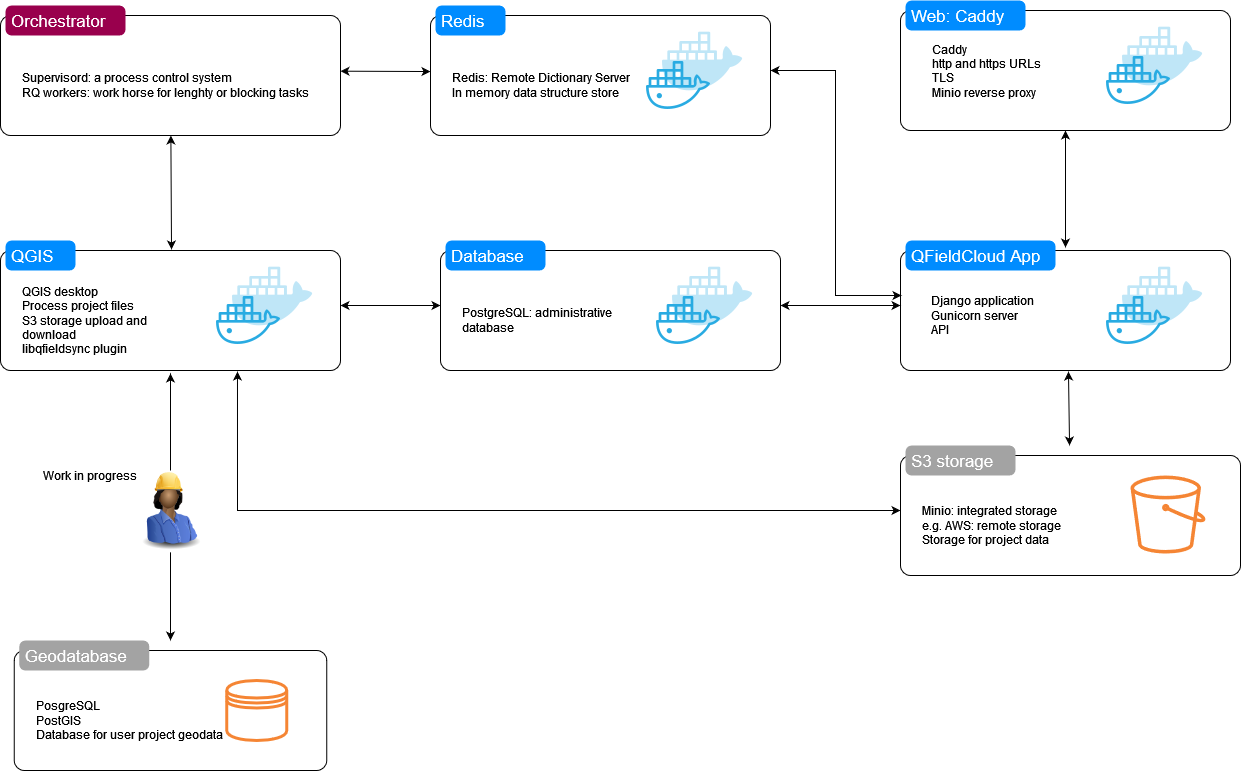
\includegraphics[width=1\textwidth]{qfielcloud_system_architecture.png}
    \caption{System architecture of QFieldCloud}
    \label{fig:system-architecture_graph}
\end{figure}

\subsection{Configuration files}

\begin{markdown}
The main configuration file is the ```.env``` file, which stores necessary environmental variables that are used to build the QFieldCloud. We have listed the environmental variables associated with a specific component under corresponding section. However, some of the variables can affect multiple components.

The ```.yml``` files are necessary for building the docker containers for the application. The ```docker-compose.yml``` is the base configuration file and the ```override.yml``` files are used to change existing components or create new ones. When building local instance, 

```docker-compose.yml```

and 

```docker-compose.override.local.yml``` are used. For server instance 

```docker-compose.yml``` 

and 

```docker-compose.override.dev.yml```

or  
```docker-compose.override.prod.yml``` is used depending on whether development or production instance is build. At the moment

`docker-compose.override.prod.yml` 

file doesn't have anything inside it except the version number.
\end{markdown}

\subsection{S3 Storage}
\begin{markdown}
QFieldCloud has a S3 storage component, which is used to store project data. The configurations allows for internal or external storage. As internal storage QFieldCloud uses integrated MinIO object storage, which is compatible with S3. The integrated storage is used by local instances. It is also possible to use an external storage like Amazon Web Services (AWS) or other service implementing the S3 API. External storage is recommended for development or production instances as then the lifetime of the data is not tied to the lifetime of Docker volumes. The S3 storage is used by other components to upload, download or modify QGIS project files and data.
\end{markdown}

\begin{minted}[breaklines]{sh}
# Environmental variables for integrated or remote S3 storage.
STORAGE_ACCESS_KEY_ID=<Used in authentication. Acts like a username.>
STORAGE_SECRET_ACCESS_KEY=<Used in authentication. Acts like a password.>
STORAGE_BUCKET_NAME=<Name of the S3 bucket>
STORAGE_REGION_NAME=<Name of the region where the bucket is hosted>
STORAGE_ENDPOINT_URL=<Internal URL to the storage endpoint>
STORAGE_ENDPOINT_URL_EXTERNAL=<Public URL to the storage endpoint>
STORAGE_BROWSER_PORT=<Port that is used to access storage browser>
\end{minted}

\subsection{Geodatabases}
\begin{markdown}
Geodatabase is a database for user project geodata. When building the software it creates internal PostGIS database. It is also possible to create multiple geodatabases through the administration page of QFieldCloud.

Geodatabase seems to be a work-in-progress feature. There doesn't seem to be any options to upload data to a geodatabase from QGIS via QFieldSync plugin. The geodatabase is also marked as work in progress according to the developers system architecture. This is most likely a future component.
\end{markdown}

\begin{minted}[breaklines]{sh}
# Environmental variables for the builded geodatabase
GEODB_HOST=<Geodatabase hostname>
GEODB_PORT=<Geodatabase port>
GEODB_USER=<Geodatabase username>
GEODB_PASSWORD=<Username password>
GEODB_DB=<Geodatabase name>
\end{minted}

\subsection{Administrative app}
\begin{markdown}
The administrative app (also known as the `app` in the `.yml`files) is the container for controlling the QFieldCloud admin application. It is a Django based service that also uses Gunicorn. Django is a Python web framework for developing database-driven Web apps. Gunicorn is a Python WSGI HTTP server, which is compatible with many web frameworks. The application delivers the [QFieldCloud REST API](https://app.qfield.cloud/swagger/) which exposes the functionality of QFieldCloud to the clients such as QField Sync or QField Dev instances. In addition to the REST API the app also offers a web admin where the QFieldCloud instance can be managed. For example, it is possible to create new users, teams and organizations  with different levels of permissions through the admin page. The main project details are also visible and can be read, modified or deleted. Through the admin page it is possible to create new geodatabases. The app also has different kinds of logs and it is possible to see user access information and other notifications.
\end{markdown}

\begin{minted}[breaklines]{sh}
# A debug setting for django in development. Should not be used in production.
DEBUG=<Enable or disable debug>

# IP address or domain name
QFIELDCLOUD_HOST=<Parameter is used to create the Django admin page and MinIO browser.>
# Settings file
DJANGO_SETTINGS_MODULE=<QFieldCloud settings file used by django>

# A secret key for django installation
SECRET_KEY=<Key used to provide cryptographic signing>

# Variables purpose is unknown
SENTRY_DSN=<???>

# Email parameters
ACCOUNT_EMAIL_VERIFICATION=<Email verification method during signup>
EMAIL_HOST=<Email host name>
EMAIL_USE_TLS=<Use TLS connection when talking to the SMTP server. True or False>
EMAIL_USE_SSL=<Use an implicit TLS connection when talking to the SMTP server. True or False>
EMAIL_PORT=<Used port>
EMAIL_HOST_USER=<Username for the SMTP server>
EMAIL_HOST_PASSWORD=<Password for the SMTP server>
DEFAULT_FROM_EMAIL=<Default email address to use>

# Project name
COMPOSE_PROJECT_NAME=<Used by docker-compose to set the project name. Used to name the container and volumes>
# Default network name
QFIELDCLOUD_DEFAULT_NETWORK=<Used when building the admin app and by workers>
# Admin URI
QFIELDCLOUD_ADMIN_URI=<Used by admin app>
\end{minted}

\subsection{postgreSQL}
\begin{markdown}
One of the QFieldCloud components is a PostgreSQL database for the administrative application. The database stores information related to the administrative app.
\end{markdown}

\begin{minted}[breaklines]{sh}
# Environmental variables for administrative application database
POSTGRES_USER=<Database username>
POSTGRES_PASSWORD=<Username password>
POSTGRES_DB=<Database name>
POSTGRES_HOST=<Database host name>
POSTGRES_PORT=<Database port>
HOST_POSTGRES_PORT=<Host port>
\end{minted}

\subsection{QGIS}
\begin{markdown}
The QGIS component is responsible for transferring data between QGIS desktop, QField Dev and QFieldCloud service. Its purpose is to process project files and data. One of the core functions is to upload or download data from the S3 storage. The component utilizes *libqfieldsync* plugin for synchronization and packaging of the data.
\end{markdown}

\subsection{Caddy}
\begin{markdown}
Caddy is a open source web server with automatic HTTPS. It is used to manage HTTP and HTTPS of the QFieldCloud service. In addition Caddy has automation for TLS. It is also used to reverse proxy MinIO. If using remote storage then the reverse proxy caddyfile should be empty.
\end{markdown}
\begin{minted}[breaklines]{sh}
# HTTP port
WEB_HTTP_PORT=<HTTP port used by Caddy and admin application>
# HTTPS port
WEB_HTTPS_PORT=<HTTPS port useb by Caddy and admin application>

# TLS option
CADDY_ACME_CA=<URL to the ACME CA's directory>
# Import caddy settings
CADDY_IMPORT_GLOB=<parameter used to import caddy settings>
\end{minted}

\subsection{Redis}
\begin{markdown}
Redis also known as Remote Dictionary Server is an open source in memory data structure store. Redis is connected to the administrative application and orchestrator components.
\end{markdown}

\begin{minted}{sh}
# Environmental variables for Redis
REDIS_PASSWORD=<Redis password>
REDIS_PORT=<Redis port>
\end{minted}

\subsection{Orchestrator}
\begin{markdown}
The QFieldCloud application is controlled by orchestrator component named supervisor. Supervisor is used to monitor and control the different processes in the application. Then there are RQ workers, which are Python processes that work in the background. They are mostly used to deal with lengthy or blocking tasks.
\end{markdown}

\subsection{Other environmental variables}
\begin{minted}[breaklines]{sh}
# Environmental variables for storing logs
LOG_DIRECTORY=<Logs directory>
TMP_DIRECTORY=<Temporary folder directory>
\end{minted}

% Eemeli
\section{Managing QFieldCloud}
The basic properties of a QFieldCloud instance can be managed either by using the management script or using the web admin page. Both those ways are shortly described here. 

\subsection{Management scripts}
\begin{markdown}
The management app contains a manage script ```manage.py``` which contains different utilities that can be used to manage the QFieldCloud instance. There are few dozen utilities but we have only needed few of those, so we'll introduce those. Documentation for most of the commands can be found from the [Django documentation](https://docs.djangoproject.com/en/3.2/ref/django-admin/) as they are common to all Django applications. All the utilities can be listed with the following command
\end{markdown}
\begin{minted}{sh}
docker-compose run app python manage.py 
\end{minted}
in the root of the project and the utilities can be used by appending the utility name after the \texttt{manage.py}.

\subsubsection{Database migrations}
Before using the application, the database migrations have to be run. They can be run by giving the command
\begin{minted}{sh}
docker-compose exec app python manage.py migrate
\end{minted}
The script will initiate the database tables that are used to store data about the projects, organizations, teams, users and other things related to the wed admin page. However, that database does not contain any project geodata.

\subsubsection{Adding a superuser}
As the QFieldCloud is currently still in beta, there are some features, such as adding the first superuser, that can be only achieved by using the manage script. The script you'll need for that is the \texttt{createsuperuser} command:
\begin{minted}{sh}
docker-compose run app python manage.py \ 
createsuperuser --username super_user \ 
--email super@user.com
\end{minted}
The script should then prompt you for the password you want to set for the user. The parameter following \texttt{--superuser} defines the name of the user and parameter after \texttt{--email} will define the email.

\subsubsection{Adding a user}
The script \texttt{createuser} actually does almost the same thing that the one in the previous section but it's not interactive meaning that you can pass the username and password as arguments instead of having to type them, and you can create users without superuser rights. It should only be used for testing purposes as storing passwords in plain text is not a good idea. Example usage is
\begin{minted}{sh}
docker-compose run app python manage.py \ 
createuser --username=test \ 
--email=test@test.com \
--password=test --superuser
\end{minted}
where \texttt{--superuser} is added only if you need to create a superuser. The result of using the command with the \texttt{--superuser} flag is exactly equivalent to the \texttt{createsuperuser} command of the Django framework.

\subsubsection{Collect static web resources}
Django contains a utility that is used to collect the static web files used on the wed admin page including all pictures and \texttt{.css} files. Without those the page looks quite weird but is still usable. You can apply the static files by running
\begin{minted}{sh}
docker-compose run app python manage.py \ 
collectstatic --noinput
\end{minted}

\subsubsection{Return service status}
The QFieldCloud has a handy utility which can be used to return the status of the different parts of the application. Currently, it returns the operating status of 'redis', 'geodb' and 'storage'. It can be called with
\begin{minted}{sh}
docker-compose run app python manage.py status
\end{minted}

\subsection{The Web admin}
The basic layout of the web admin can be seen in Fig \ref{fig:webAdmin}. The web admin allows managing every aspect of the QFieldCloud instance including adding (super)users, organizations, projects and teams and assigning projects to teams, users and organizations. Organizations are effectively the same as users so they can be assigned projects but they also allow adding teams under the organization. The teams can contain users from multiple organizations and the users can belong to many teams. The \emph{Invitations} view can be used to invite more people to your service but it requires setting the email environmental variables correctly, which we never did.

By clicking the different links on the home page of the web admin, you can get more detailed view. For example, by clicking the \emph{Deltas} you can return the view where the Deltas (i.e. the changes) can be applied and conflicts between different concurrent edits can be solved. \emph{Jobs: Process QGIS project file} is a very useful view to check if your upload of a QGIS project has actually worked. 

\begin{figure}[htb]
    \centering
    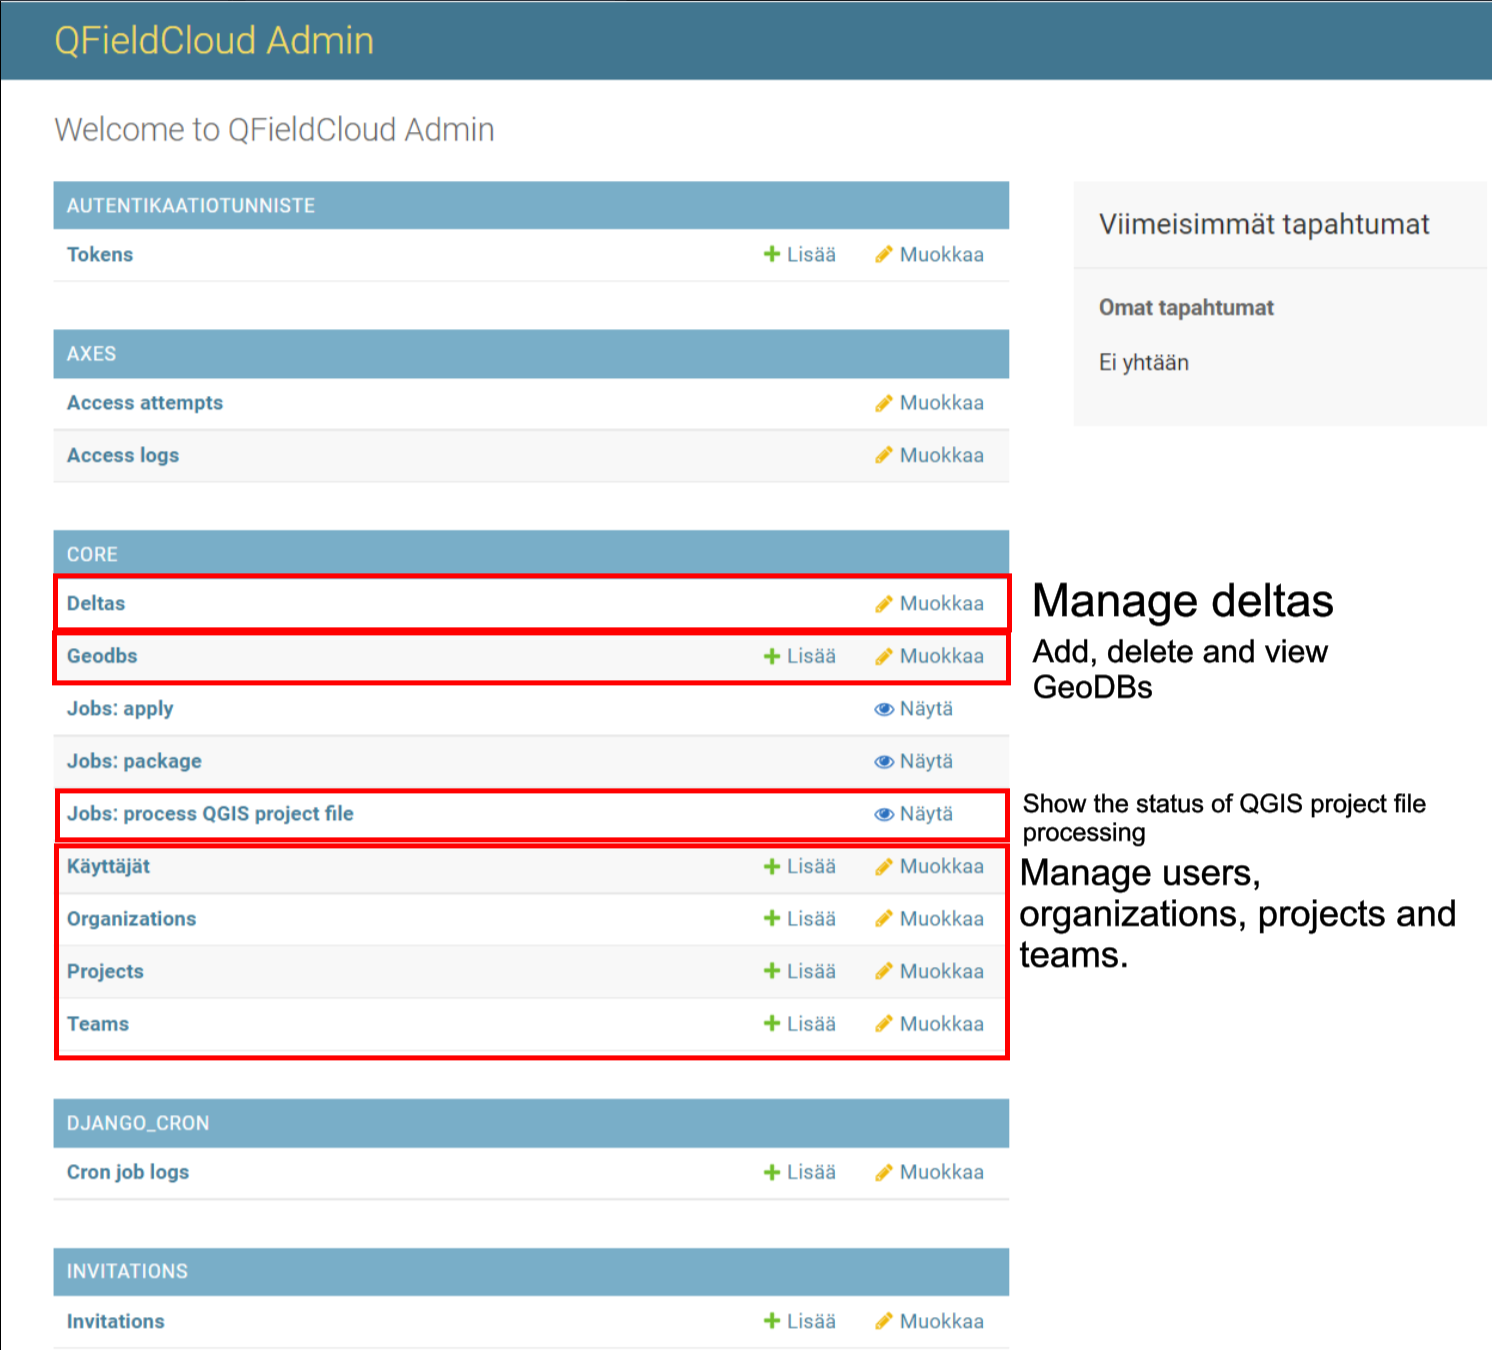
\includegraphics[width=1\textwidth]{web_admin_page.PNG}
    \caption{The web admin view with some captions for the most useful components}
    \label{fig:webAdmin}
\end{figure}
% Ngoc
\section{The installation and configuration of client software}

\subsection{QField Sync plugin and QField Dev mobile application}

\textbf{QField Sync}

We used the QField Sync plugin v4.0.0-beta16 in the project. The used plugin version was experimental, and there is already a newer experimental version as well. You can download the latest version from here:
\url{https://plugins.qgis.org/plugins/qfieldsync/}. After downloading the plugin, you have the plugin as zip-file. To install the plugin, open QGIS and click on 'Plugins' tab and you can see under the tab the option 'Manage and Install Plugins...' which you should click. This will open the 'Plugins' window and choose 'Install from ZIP' from the left panel. Then you should browse and select the downloaded zip-file in order to install the plugin to QGIS. When the QFieldCloud login dialog pops up off the screen, you should double-click the blue bug in order to see the server URL input field which you can type in your URL (see Figure \ref{fig:login-qfieldsync}).


\begin{figure}[H]
    \centering
    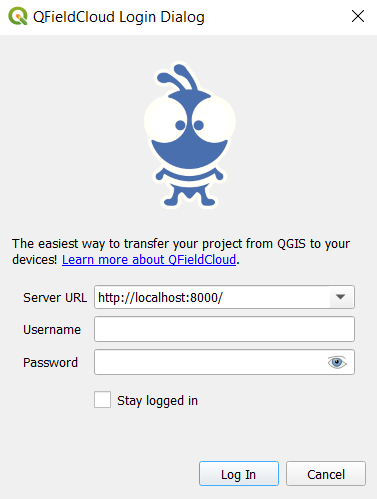
\includegraphics[width=0.5\textwidth]{login-qfieldsync.png}
    \caption{Screenshot of the login window}
    \label{fig:login-qfieldsync}
\end{figure}

\textbf{QField Dev}

We used QField for QGIS early access version in the project. The application is currently only available on Android devices, and it can be downloaded from Google Play. When you open QFieldCloud, you can see from the main menu the option 'QFieldCloud projects' where you can login QFieldCloud. Remember to double-click the blue bug in order to change the server URL. 


\section{Working with a cloud project on QGIS}
% Eemeli
\subsection{Actions and the different types of layers}
\begin{markdown}
The actions related to QFieldCloud operations are best explained in the official [documentation](https://github.com/opengisch/qfieldcloud/blob/master/docs/system_documentation.org#qgis-project). The actions are
- OFFLINE
- NO_ACTION
- REMOVE
- COPY
- KEEP_EXISTING
and they are saved in the QGIS project file as a \texttt{customProperty} under the \texttt{QFieldSync/action} key. Each layer in the project file can have its own type of action defined independent of the other layers.

QFieldCloud makes a distinction between file-based layers, such as GeoPackages, and database layers, such as PostGIS layers. The actions work differently based on whether the layer is file based or a database layer and also by which actor, (QFieldSync, QFieldCloud, QField)  is handling the layer. QField application will try to directly access the data source with database layers on ```NO_ACTION```, but on ```OFFLINE``` it will create and push a Delta file. 

To use the live editing of the database, is has to be accessible in the internet and the database connection strings including \textbf{plain text passwords and username} should be included in the QGIS project file. This should be configured by QFieldSync if you set a layer as directly accessed layer. It's important to notice that you cannot set the connection to the database with the QGIS authorization configuration but you have to use the basic authentication, as otherwise the \emph{auth} configuration in the connection string will point to an authentication in the local authentication database not accessible to the outside world. 
\end{markdown}


\subsection{The synchronization modes}
A QGIS project can be a \texttt{.qgs} or \texttt{.qgz} file that can be created on QGIS Desktop, and uploaded as a cloud project to QFieldSync-plugin. It is important to configure the project properties since the configurations determine how QFieldCloud or QField will handle each layer.

In QFieldCloud tab, you can choose 'Prefer online layers' or 'Prefer offline layers' to apply the configurations for all layers. Or you can determine the configurations by choosing an option for one layer at a time in the column 'Action' (see Fig \ref{fig:qgis-create-cloud-project}). The options are 'Directly access data source', 'Offline' or 'Remove from project'.

\begin{figure}[H]
    \centering
    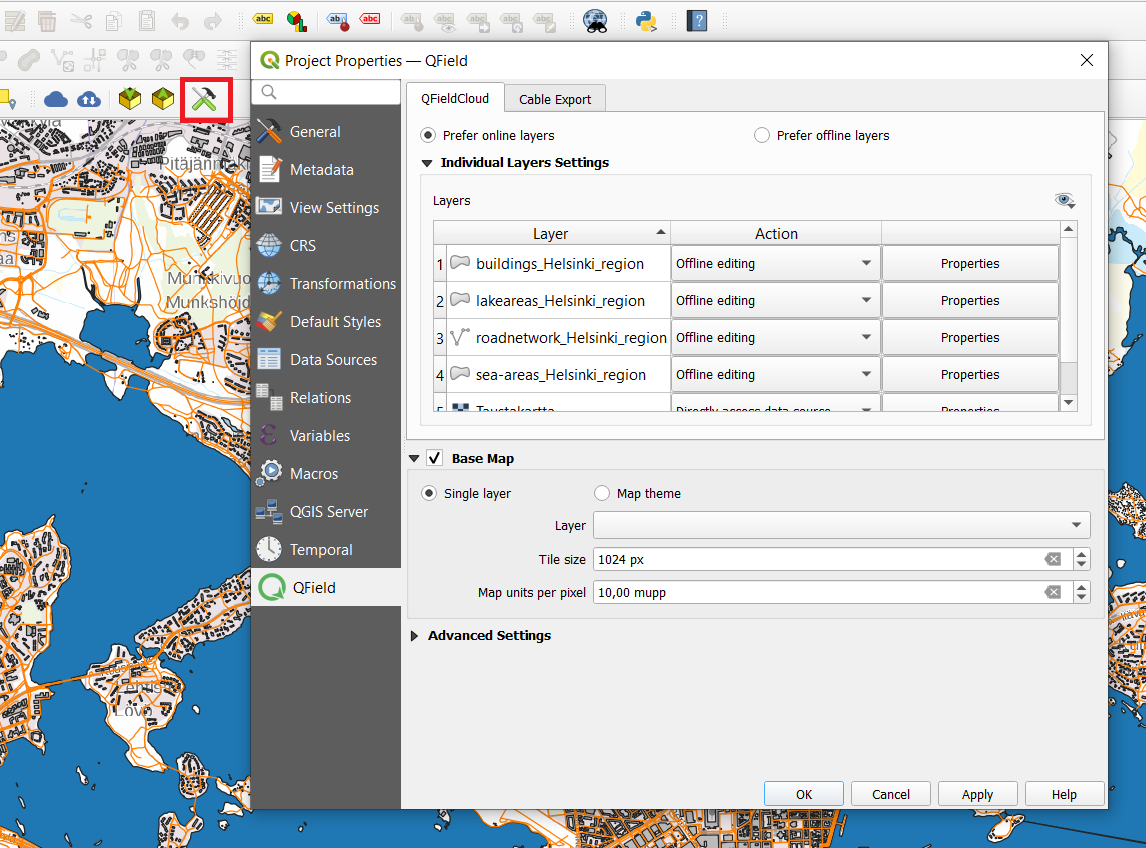
\includegraphics[width=1\textwidth]{qgis-project-properties.png}
    \caption{The configurations of the layers}
    \label{fig:qgis-create-cloud-project}
\end{figure}

%\subsection{Downloading the data}

\subsection{Sending a project to the cloud}
There are two ways to create a cloud project on QGIS. The first option is to convert the open project to cloud project, and the second option is to create a new empty cloud project (see Fig \ref{fig:qgis-create-cloud-project}).

\begin{figure}[H]
    \centering
    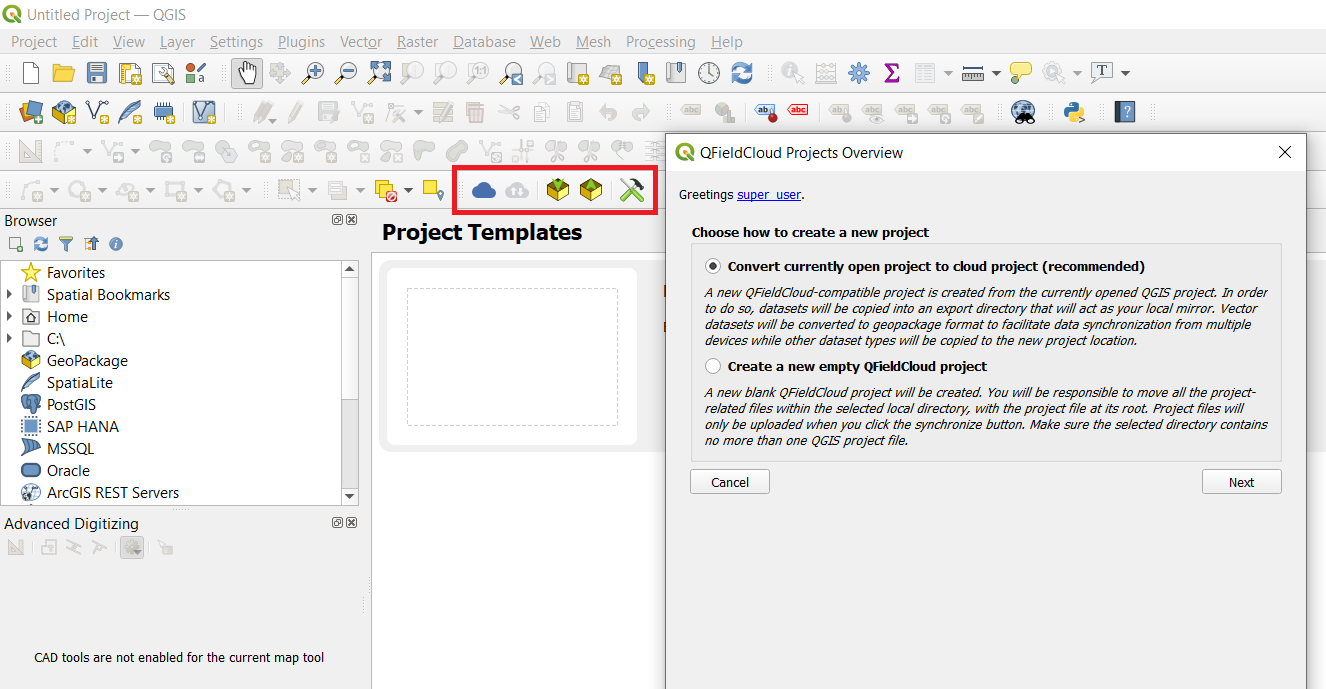
\includegraphics[width=1\textwidth]{qgis-create-cloud-project.png}
    \caption{The two different options for creating a cloud project}
    \label{fig:qgis-create-cloud-project}
\end{figure}

If you choose 'Convert currently open project to cloud project', it will upload the project files to the cloud, and you can see the project from QFieldCloud admin site and QField mobile app.

When you choose the option 'Create a new empty cloud project', you need to open the QFieldCloud projects overview and select the synchronization icon in the left bottom corner of the window (see Fig \ref{fig:qgis-create-empty-project}) for uploading files to the empty project.

\begin{figure}[H]
    \centering
    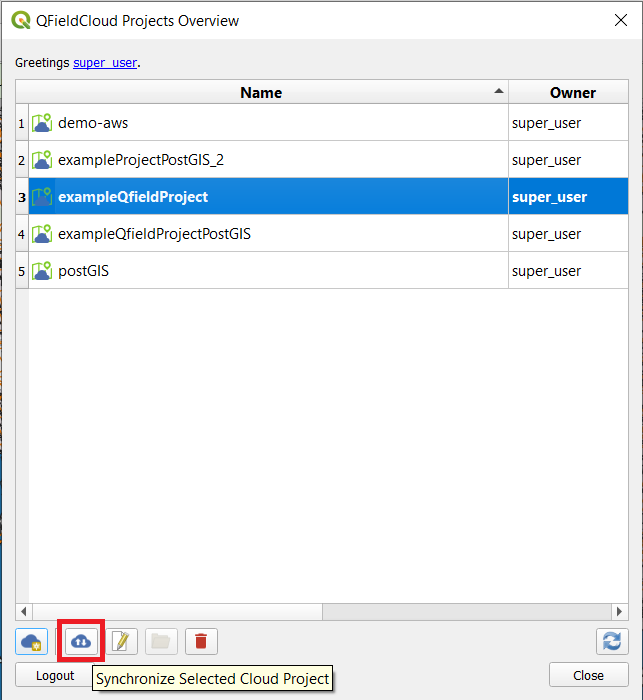
\includegraphics[width=1\textwidth]{qgis-create-empty-project.png}
    \caption{Upload the current layers to the empty cloud project}
    \label{fig:qgis-create-empty-project}
\end{figure}

Then, the synchronizing project window view will pop, and you can choose what to upload to the empty cloud project (see Fig \ref{fig:qgis-create-cloud-project-1}). Finally, clicking 'Upload Project' will synchronize the files to the cloud.

\begin{figure}[H]
    \centering
    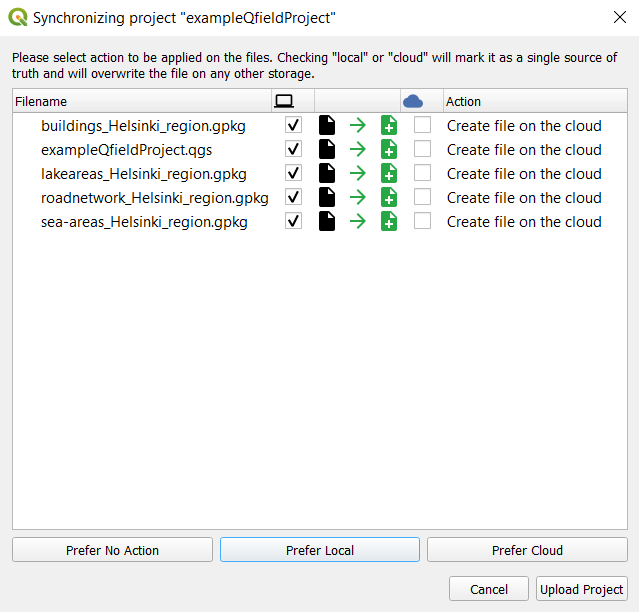
\includegraphics[width=1\textwidth]{qgis-create-empty-project-1.png}
    \caption{Choose the wanted project files to be uploaded}
    \label{fig:qgis-create-cloud-project-1}
\end{figure}

\subsection{Synchronization of a cloud project to QGIS}

Click the QFieldSync's cloud icon from the QGIS toolbar to open the QFieldCloud project overview. Choose the wanted project, and click the synchronization icon in the left bottom corner of the window (see Figure \ref{fig:download}).

\begin{figure}[H]
    \centering
    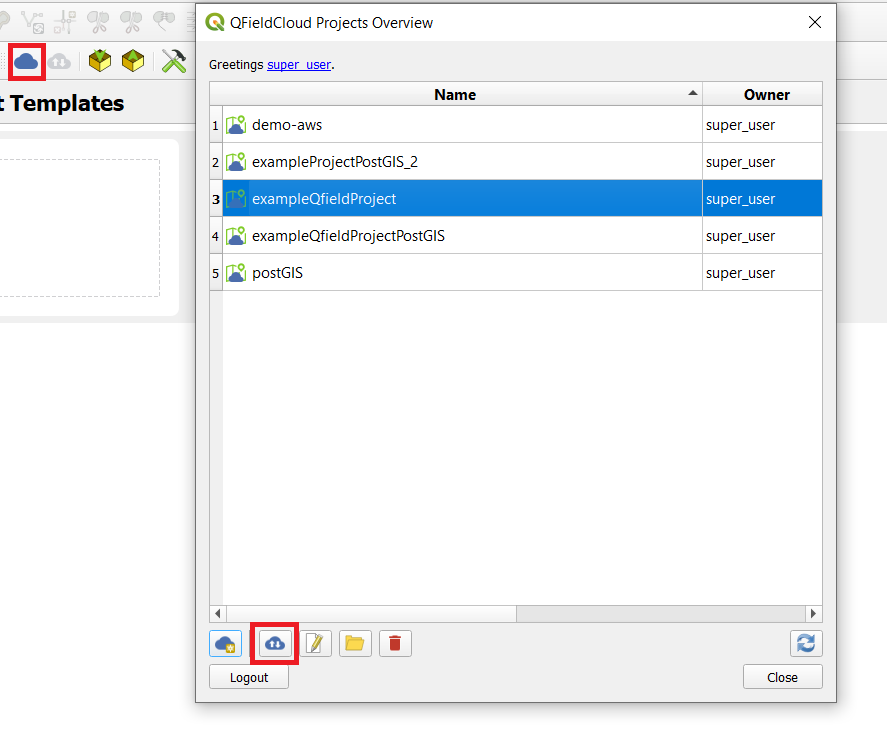
\includegraphics[width=1\textwidth]{download-project.png}
    \caption{Select the wanted cloud project to download}
    \label{fig:download}
\end{figure}

Then you have to choose 'Prefer Cloud', and it will replace the local version. You can select which files you want to synchronize by ticking the boxes (see Figure \ref{fig:download-1}). When the selection is done, click 'Upload Project'.

\begin{figure}[H]
    \centering
    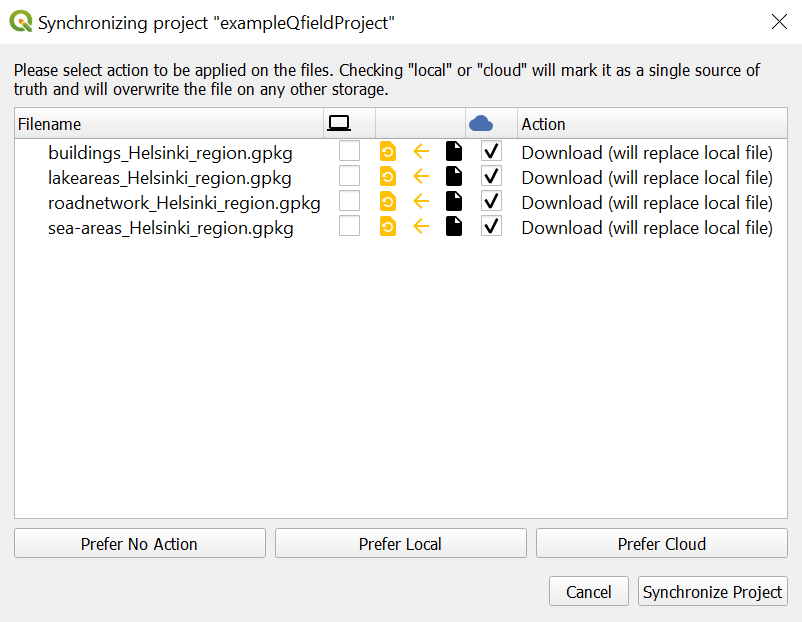
\includegraphics[width=1\textwidth]{qfieldcloud_download.PNG}
    \caption{Choose the files from the cloud project}
    \label{fig:download-1}
\end{figure}

If you do not have the local files of the project, the synchronization action differs from the previous situation (see Figure \ref{fig:download-2}). It will download the selected files to your machine.

\begin{figure}[H]
    \centering
    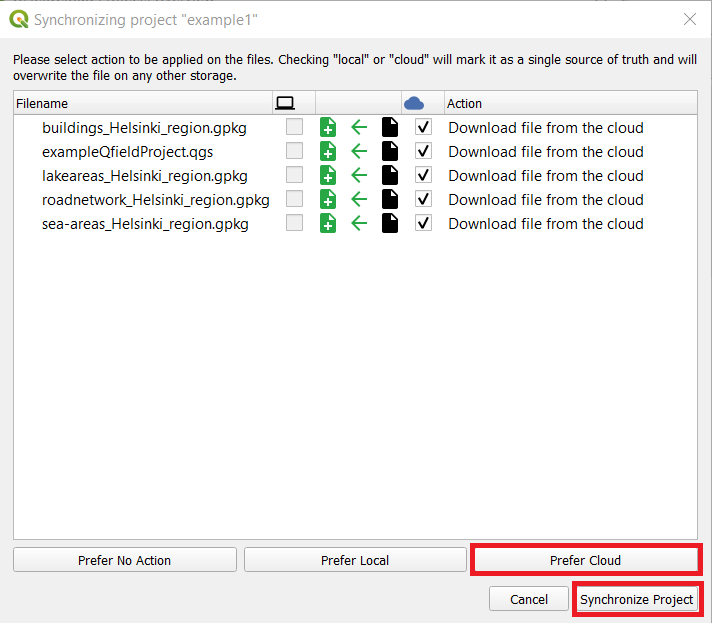
\includegraphics[width=1\textwidth]{dl-project-2.png}
    \caption{Choose the files from the cloud project}
    \label{fig:download-2}
\end{figure}

%\subsection{Preparing a project in QGIS}





\section{Working with a cloud project on the mobile app}
The left screenshot, that can be seen in the Figure \ref{fig:login-qfield}, is the main view of the QField app. In order to the login QFieldCloud, you need to press 'QFieldCloud projects'-button. Then, the app will take you to login view where you can type your server URL and account information. To get the server URL visible, you need to double-click the blue bug. After a successful login, you are able to see your accounts projects.

\begin{figure}[H]
    \centering
    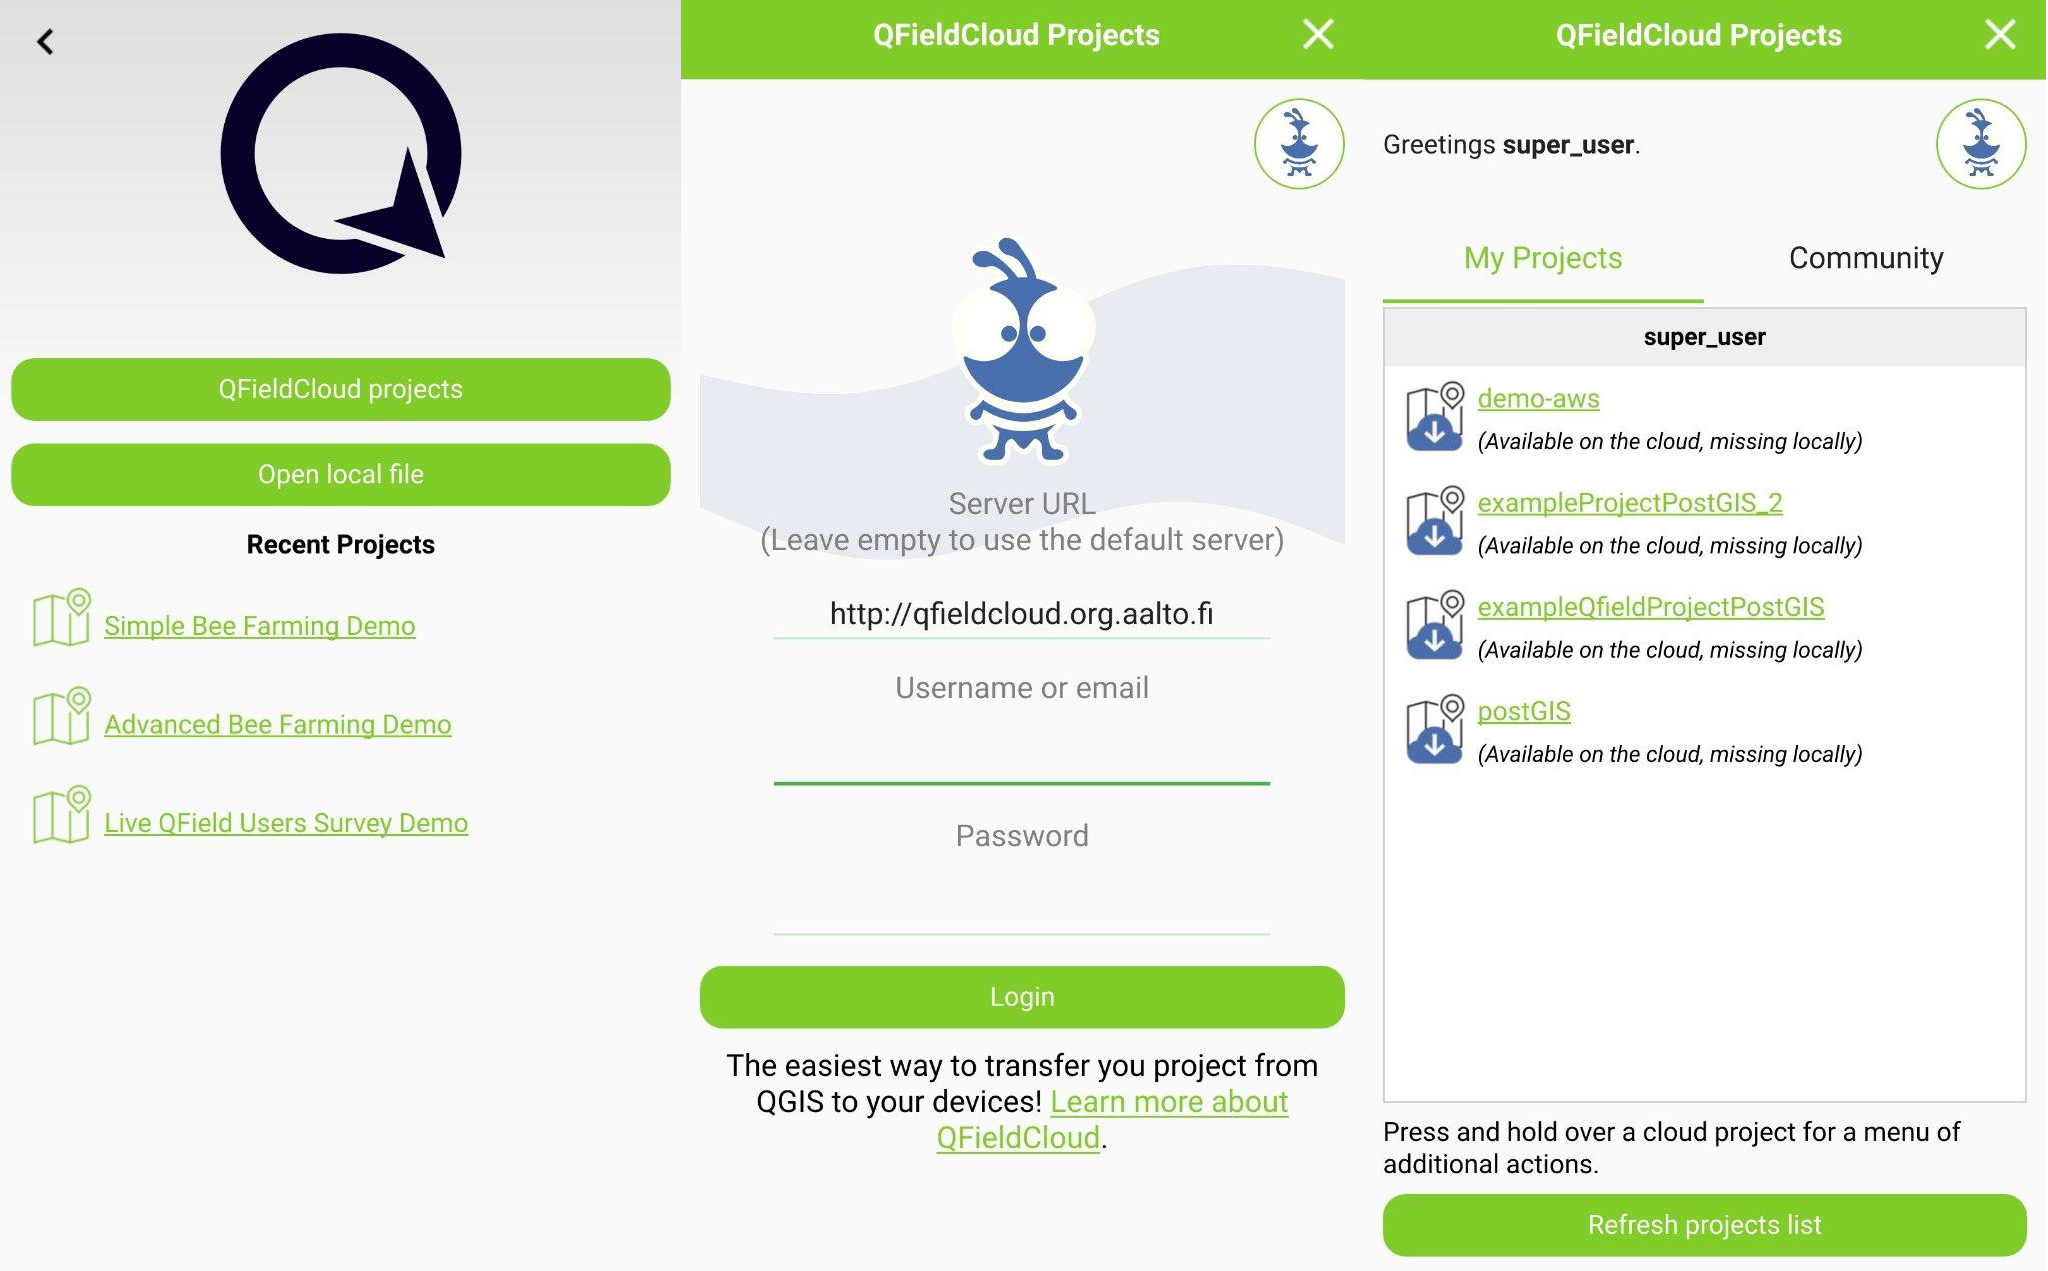
\includegraphics[width=1\textwidth]{qfield-login.png}
    \caption{Screenshots of QField app}
    \label{fig:login-qfield}
\end{figure}


% Ngoc
\section{Results}
The project did not manage to create a QFieldCloud demonstration with the most important functions working. This section will go through which components of the QFieldCloud work and which do not work. 

\subsection{The working parts}
\begin{markdown}
- Creating a super user
- Databases can be accessed via SQL client
- The connection between QFieldCloud and QGIS with QFieldSync and mobile device through QField works
- Creating cloud projects in QGIS to the QFieldCloud
- The storage of local and server instance works properly, and it is possible to upload the data to internal (MiniO) and external storage (AWS S3). It has been validated that the project upload is complete through downloading it manually from the storages.
- The Django admin site works as it should. It is possible to manage users, teams, organizations and projects. Also, it is possible to create geodatabases through the admin page.
\end{markdown}

\subsection{Some issues and probable solutions}
\begin{markdown}
- Converting the currently open project to a cloud project does not work consistently
    - You can, however, achieve the same result by creating a new project, configuring it as a cloud project, synchronizing it to cloud and adding the data after that.
- Synchronizing projects from QFieldCloud does not work, In other words, it is not possible to import the projects to QGIS and QField.
    - We did not find a solution although that's probably our own incompetence 
- HTTPS is not working correctly, as the root certificate is not from a trusted certificate authority.
    - In QFieldSync you can save an exception for the certificate, which will let it use the HTTPS.
    - You can add the TLS certificate (certificate and private key) inside the caddy-container with docker-volumes. The TLS parameter inside the Caddyfile can then be used to access those files and configure the certification in the correct manner. (Not tested)
    - The newest version of QFieldCloud removed Caddy, uses NGinx instead and has a better way to add the certificate. (Not tested)
- File transfer in QFieldSync fails mid-transfer.
    - No known solution. Sometimes uploading one layer at the time will work. 
- The current user will be logged out abruptly in QFieldSync
    - No known solution. Likely has something to do with the lifetime of authentication tokens or cookies.
- *AssertionError* when adding a new project on QFieldSync
    - No certain solution. Checking if the local directory contains the file path that is used by the project and adding those directories by hand will sometimes work. 
- *IndexError* when adding an Organization with `Account Type = Pro` in the web admin. 
    - Select 'community' instead. It will actual create a 'pro' user anyway.
\end{markdown}

% Eemeli
\section{Discussion and conclusions}
The aim of the project was to investigate the state of the QFieldCloud by conducting Proof-of-Concept testing. During the course of the project we set the QFieldCloud on our own virtual machines, on a server provided by Aalto University, and attempted to synchronize geospatial data to the cloud using QFieldSync plugin on QGIS. 

From a practical standpoint, the project wasn't succesful as we never managed to set up a working instance and therefore we could not test the whole product stack of QGIS + QFieldSync, QFieldCloud and QField as we were supposed to do. However, what we can conclude from the project is that although some of the problems we faced during the project can be products of our own incompetency, the QFieldCloud has issues. 

Documentation on how to set up some things on the server is missing completely, and some is out-of-date. For example, the documentation mentions Geodatabases but never clarifies where and how they are utilized, except for the system documentation diagram that has not been updated since March, 2021. Despite that the system has seen some minor updates and one major update, which made some parts of this report already obsolete.

What we could get working, however, was promising. We could get files to the cloud using the QFieldSync and we could see those files appear to the S3 storage. We were able to manage users, organizations, teams and projects using the web admin. However, the utility of QFieldCloud comes down to whether OPENGIS.CH can solve the problems.

\begin{markdown}
Using standard Docker for this kind of complex service is also slightly questionable and makes the data hard to manage. For an actual production build, it would be advisable to host the databases outside the containers and use technologies such as [Docker Swarm](https://docs.docker.com/engine/swarm/swarm-tutorial/) or convert the service to Kubernetes cluster using [Kompose.io](https://kompose.io/). 
\end{markdown}

Although the synchronization from the cloud is probably easy to solve by professionals, at the current state, the QFieldCloud is not ready for production. Even the functions that we got working, work quite inconsistently. For example, the current user can be logged out in the middle of file transfer and sometimes the transfer aborts without a warning especially if multiple layers are uploaded at once. Additionally, there are some bugs here and there which may not render the application unusable but are frustrating to the user.     

%Moving on from standard Docker

%Including an external \texttt{.md} file:

%\markdownInput{example.md}

\end{document}
